\documentclass[11pt]{article}
\usepackage[utf8]{inputenc}
\usepackage{amsmath}
\usepackage{amsfonts}
\usepackage{amssymb}
\usepackage{graphicx}
\usepackage[super]{nth}
\usepackage{amsthm}
\usepackage{bm}
\newtheorem{theorem}{Theorem}
\newtheorem{objective}{Objective}
\newtheorem{model}{Model}
\usepackage{xcolor}
\definecolor{light-gray}{gray}{0.95}
\newcommand{\code}[1]{\colorbox{light-gray}{\texttt{#1}}}
\usepackage{listings}

\usepackage[authoryear]{natbib}


\makeatletter
\renewcommand{\maketitle}{
\begin{center}

\pagestyle{empty}

{\Large \bf \@title\par}
\vspace{1cm}

{\LARGE Marcel Gietzmann-Sanders}\\[1cm]

STAT641 - Bayesian Statistics \\
University of Alaska Fairbanks


\end{center}
}\makeatother


\title{Implementing a BYM Model in Stan to Fit Boston Housing Price Data}

\date{2024}
\setcounter{tocdepth}{2}
\begin{document}
\maketitle
\tableofcontents
\newpage 

\section{Data on Boston Housing Prices in 1978}

For this study we'll be using a dataset originally published in 1978 on housing prices in Boston, Massachusetts (\cite{origin}). This data was made accessible through the \code{spData} package in R (\cite{spdata}). Specifically, it contains median house prices and potential covariates for 506 tracts in the Greater Boston Area. Fig. \ref{fig:prices} shows the median price per tract of land. It should be understood that this data is censored and median values over \$50,000 are capped. A full list of covariates can be found in the documentation for the \code{boston} dataset in \code{spData}. What we wish to understand is which of these covariates are indeed related to housing prices after being added to a spatial bayesian model. \newline

Starting with some exploratory data analysis we identified four covariates of particular interest. Crime rates per capita, average number of rooms per dwelling, weighted distance to employment centers, and the nitric oxide concentrations per town. 

First, as the distribution of values is right skewed (and following in the footsteps of (\cite{book})) we took as our target variable the logarithm of the median house value per tract instead of the median value itself. Fig. \ref{fig:price_dist} shows the distribution of our target. 



Fig. \ref{fig:crime} shows the relationship between per capita crime rate and our target. There appears to be a clear negative relationship between then two and a rather wide spread of values in and around 0. 

Fig. \ref{fig:rooms} shows how our target varies with the average number of rooms per dwelling in each tract. Here we can see a strong positive relationship between the two which makes a great deal of sense. 

In Fig. \ref{fig:employment} we see what looks to be a similar positive relationship between the logarithm of the average weighted distance to employment centers and our target. However this relationship is not as clear or strong as the one between our target and the number of rooms per dwelling. 

Finally Fig. \ref{fig:nox} shows us the relationship between nitric oxide concentrations in parts per million and our target with a somewhat spurious negative relationship. 

\newpage


\section{Defining the Model}

We will be using a variant of the Besag-York-Mollié (BYM) model (\cite{book})(\cite{bymstan}). In this model we assume that we have an observations of our target variable $Y_i$ (log median housing value in our case) for each tract $i$. Furthermore we assume our $Y_i$ can be modeled as a normal distribution:

$$Y_i \sim Normal(\mu_i, \sigma^2)$$

where it is the $\mu_i$ that will be a function by our covariates. Specifically:

$$\mu_i= \beta_0 + \vec{\beta} \vec{x_i} + \sigma_r\left( \sqrt{\rho}\phi_i + \sqrt{1-\rho}\theta_i \right)$$

where $\beta_0$ is our intercept, $\vec{\beta}$ are the coefficients for our models effects from each covariate, $x_i$ are our covariates corresponding to tract $i$, $\phi_i$ and $\theta_i$ are spatial and random effects respectively, and $sigma_r$ and $\rho$ allow us to control the effect of the random variables as well as the degree to which our model has spatial and/or unstructured noise (if $\rho=1$ we have only spatial structure whereas if $\rho=0$ it is totally unstructured). 

For our more straightforward priors we will have:

$$\beta_0 \sim Normal(0,1)$$
$$\beta_i \sim Normal(0,1)$$
$$\theta_i \sim Normal(0,1)$$
$$\sigma_r \sim Uniform(0,1)$$
$$\rho = \frac{e^{r}}{1 + e^{r}}, r\sim Normal(0,1)$$

In the initial experimentation with this model we also had the prior:


$$\sigma \sim Normal(0,1)$$

but consistently found $\sigma \approx 0$. Therefore going forward we simply assume $\sigma=0.01$ in order to not over complicate the sampling. 

Our spatial terms $\phi_i$ are a little more complicated. \newline

Each spatial interaction term $\phi_i$ is modeled as conditional on the other terms:

$$\phi_i | \phi_j \sim N\left(\sum_j w_{ij}\phi_j, \sigma^2  \right), i\neq j$$

This gives us a conditional autoregressive model (CAR). A key result that Besag proved (\cite{besag}) is that the joint distribution $\bm{\phi}$ ends up being multivariate normal random variable centered at 0

$$\vec{\phi}\sim N(0, Q^{-1})$$

where $Q=D(I-\alpha A)$. $D$ is a diagonal "neighbors" matrix (each element on the diagonal is the number of neighbors unit $i$ has), $A$ is an adjacency matrix where if $i,j$ are neighbors then the $i,j$ element is 1, and $\alpha$ lets us control spatial dependence. This results in a log probability density of $\vec{\phi}$ which is proportional to (\cite{bymstan}):

$$\frac{n}{2}\log{(\det{Q})}-\frac{1}{2}\vec{\phi}^T Q \vec{\phi}$$

Given $\det{Q}$ is a constant and MCMC samplers compute the log probability up to a proportionality constant (\cite{bymstan}) the first term drops out of the computation thereby reducing the computational intensity of this evaluation. 

In our case, as we will be following the stan implementation from the paper (\cite{bymstan}) we will be setting $\alpha=1$ and thereby get an intrinsic conditional autoregressive model (ICAR) in which $Q$ reduces to $D-A$. With an ICAR model each $\phi_i$ is distributed with a mean equal to the average of its neighbors. If we additionally assume that $\vec{\phi}$ is centered at zero with common variance 1, then the joint probability of $\vec{\phi}$ becomes (\cite{bymstan}):

$$p(\vec{\phi})\propto \exp{\left( -\frac{1}{2} \sum_{i\sim j} (\phi_i - \phi_j)^2 \right)}$$

where $i \sim j$ indicates that $i$ and $j$ are neighbors. This then is our prior for the $\phi_i$ - an ICAR model centered at $0$ with common variance $1$. 

\newpage

\section{Fitting the Model}

After computing the appropriate features (covariates and neighbors arrays) we fit our model using \code{rstan} (\cite{rstan}) in the \code{R} programming language (\cite{R}). Each model was fit with 4 chains and 20,000 iterations per chain. 20,000 was selected to ensure each parameter of interest had at least 1,000 effective samples. \newline

Two models were fit, one with the crime rates feature and one without (see section \ref{results}). The trace plots for the former can be found in figures \ref{fig:tbetas}-\ref{fig:tlogit_rho} and the trace plots for the latter are in figures \ref{fig:tbetas2}-\ref{fig:tlogit_rho2}. Densities are in figures \ref{fig:dbetas}-\ref{fig:dlogit_rho} and \ref{fig:dbetas2}-\ref{fig:dlogit_rho2} respectively. The order of features was crime, rooms, distance, and nox for the full model and rooms, distance, and nox for the limited model. \newline

See section \ref{stanmodel} for the \code{stan} model itself and section \ref{inputs} for the \code{R} code used to build inputs. 


\section{Results} \label{results}


\begin{center}
\begin{tabular}{ c  | c | c | c | c | c | c}
\hline
 Parameter & 95\% CI & Mean & SD & SE & $\hat{R}$ & $n_{EFF}$ \\ 
 \hline
 $\beta_0$ & 2.127, 2.394 & 2.260 & 0.197 & 0.002 & 1.000 & 7584 \\
 $\beta_{CRIM}$ & -0.009, -0.007 & -0.008 & 0.001 & $\approx 0$ & 1.000 & 40517  \\
 $\beta_{RM}$ & 0.237, 0.255 & 0.246 & 0.014 & $\approx 0$  & 1.000 & 27304 \\
 $\beta_{\log{(DIS)}}$ & -0.166, -0.054 & -0.111 & 0.083 & 0.002 & 1.002 & 1635 \\
 $\beta_{NOX}$ & -1.236, -0.970 & -1.102 & 0.196 & 0.002 & 1.000 & 11994 \\
 $\sigma_r$ & 0.342, 0.363 & 0.352 & 0.016 & $\approx 0$ & 1.000 & 7770 \\
$\rho$ & 0.941, 0.966 & 0.952 & 0.019 & $\approx 0$ & 1.001 & 3800 \\
\hline
\end{tabular}
\end{center}

Given the very small value on $\beta_{CRIM}$ we also trained a model without that feature present. 

\begin{center}
\begin{tabular}{ c  | c | c | c | c | c | c}
\hline
 Parameter & 95\% CI & Mean & SD & SE & $\hat{R}$ & $n_{EFF}$ \\ 
 \hline
 $\beta_0$ & 2.040,  2.312 & 2.176 & 0.202 & 0.002 & 1.000 & 6716 \\
 $\beta_{RM}$ & 0.237, 0.257 & 0.247 & 0.015 & $\approx 0$ & 1.000 & 20504 \\
 $\beta_{\log{(DIS)}}$ & -0.116, 0.002 & -0.057 & 0.088 & 0.002 & 1.002 & 1350 \\
 $\beta_{NOX}$ & -1.267, -0.992 & -1.130 & 0.204 & 0.002 & 1.001 & 8552 \\
 $\sigma_r$ & 0.361, 0.382 & 0.371 & 0.016 & $\approx 0$ & 1.001 & 7265 \\
 $\rho$ & 0.953, 0.973 & 0.962 & 0.016 & $\approx 0$ & 1.001 & 2997 \\
 \hline
\end{tabular}
\end{center}

Here we can see that the standard errors are small and the $\hat{R}$ values are all below 1.05. In addition the traceplots all look grassy (Figures \ref{fig:tbetas2}-\ref{fig:tlogit_rho2}). Therefore it does not seem there is much evidence to suggest a lack of convergence. \newline

The results themselves are quite interesting. We can see we have the positive relationship between number of rooms per dwelling and our median housing price with $\beta_{RM}$ being positive. It is also interesting to note just how inconsequential $\beta_{CRIM}$ was when we took into account the other features and the spatial correlations among tracts (through the $\phi_i$). We can also see that contrary to our original view, there is in fact a negative relationship between the distance to centers of employment and median housing prices per tract ($\beta_{\log{DIS}}$). However the relationship is also quite small. Finally there is a strong negative relationship between nitric oxide levels and housing prices. 

It is also quite interesting to note that $\rho$ ended up being very nearly one meaning our noise was almost entirely spatially structured. \newline

Given the relatively small value of $\beta_{\log{DIS}}$ and the fact that its 95\% credible interval crosses 0, we also looked at the bayes factor for the hypothesis that $\beta_{\log{DIS}}<0$. The posterior odds were found to be $\approx 2.92$ and given the prior was a normal distribution centered at 0 our prior odds are simply $1$ giving us a bayes factor of $2.92$. Therefore we are just shy of weak evidence for this parameter being non-zero. \newline

All in all then, it seems like our two strongest determinants of housing price are the number of rooms per dwelling and the levels of pollution as indicated by nitric oxide levels. Beyond that we also found that there was significant spatial structure in the median housing prices. All of these conclusions seem reasonable given the context. 

\newpage


\section{The Stan Model} \label{stanmodel}

\begin{lstlisting}[language=C++, basicstyle=\small]

functions {
    real icar_normal_lpdf(vector phi, int N, int[] node1, int[] node2) {
        return -0.5 * dot_self(phi[node1] - phi[node2]) 
            + normal_lpdf(sum(phi) | 0, 0.001 * N);
    }
}
data {
    int<lower=0> N; // number of tracts
    int<lower=0> N_edges; // number of unique edges
    int<lower=1, upper=N> node1[N_edges]; // start of edge
    int<lower=1, upper=N> node2[N_edges]; // end of edge
    int<lower=1> K; // number of covariates
    matrix[N, K] x; // design matrix
    real y[N]; // target
}
parameters {
    real beta0;
    vector[K] betas;

    real logit_rho;

    vector[N] phi;
    vector[N] theta;

    real<lower=0> sigma_r;
}
transformed parameters {
    real<lower=0, upper=1> rho = inv_logit(logit_rho);
    vector[N] convolved_re = sqrt(rho) * phi 
                                + sqrt(1 - rho) * theta;
}
model {
    y ~ normal(beta0 + x * betas + convolved_re * sigma_r, 0.01);
    target += icar_normal_lpdf(phi | N, node1, node2);
    beta0 ~ normal(0, 1);
    betas ~ normal(0, 1);
    logit_rho ~ normal(0, 1);
    theta ~ normal(0, 1);
    sigma_r ~ uniform(0, 1);
}

\end{lstlisting}

Note the term \verb+normal_lpdf(sum(phi)|0,0.001*N)+ used to center $\vec{\phi}$ at zero (\cite{bymstan}). 


\section{Building Inputs} \label{inputs}

\begin{lstlisting}[language=R, basicstyle=\small]
library(sf)
library(spData)
library(spdep)

map <- st_read(
    system.file("shapes/boston_tracts.shp", package = "spData"), 
    quiet = TRUE
)
map$log_median_value <- log(map$MEDV)

# build neighbors arrays
nb <- poly2nb(map)
N = length(map$MEDV)
node1 = c()
node2 = c()
for (i in 1:N) {
    for (j in nb[[i]]) {
        if (j > i) {
            node1 = c(node1, i)
            node2 = c(node2, j)
        }
    }
}
N_edges = length(node1)

# build target and covariates
y = map$log_median_value
x = cbind(map$CRIM, map$RM, log(map$DIS), map$NOX)
K = dim(x)[2]
\end{lstlisting}

Packages used - \code{spData} (\cite{spdata}), \code{sf} (\cite{sf1} \cite{sf2}), \code{spdep} (\cite{spdep1} \cite{spdep2} \cite{spdep3} \cite{spdep4})

\newpage

\section{Bibliography}

\bibliographystyle{apalike}
\bibliography{reference}

\newpage



\section{Figures}

\begin{figure}[h!] 
  \centering
  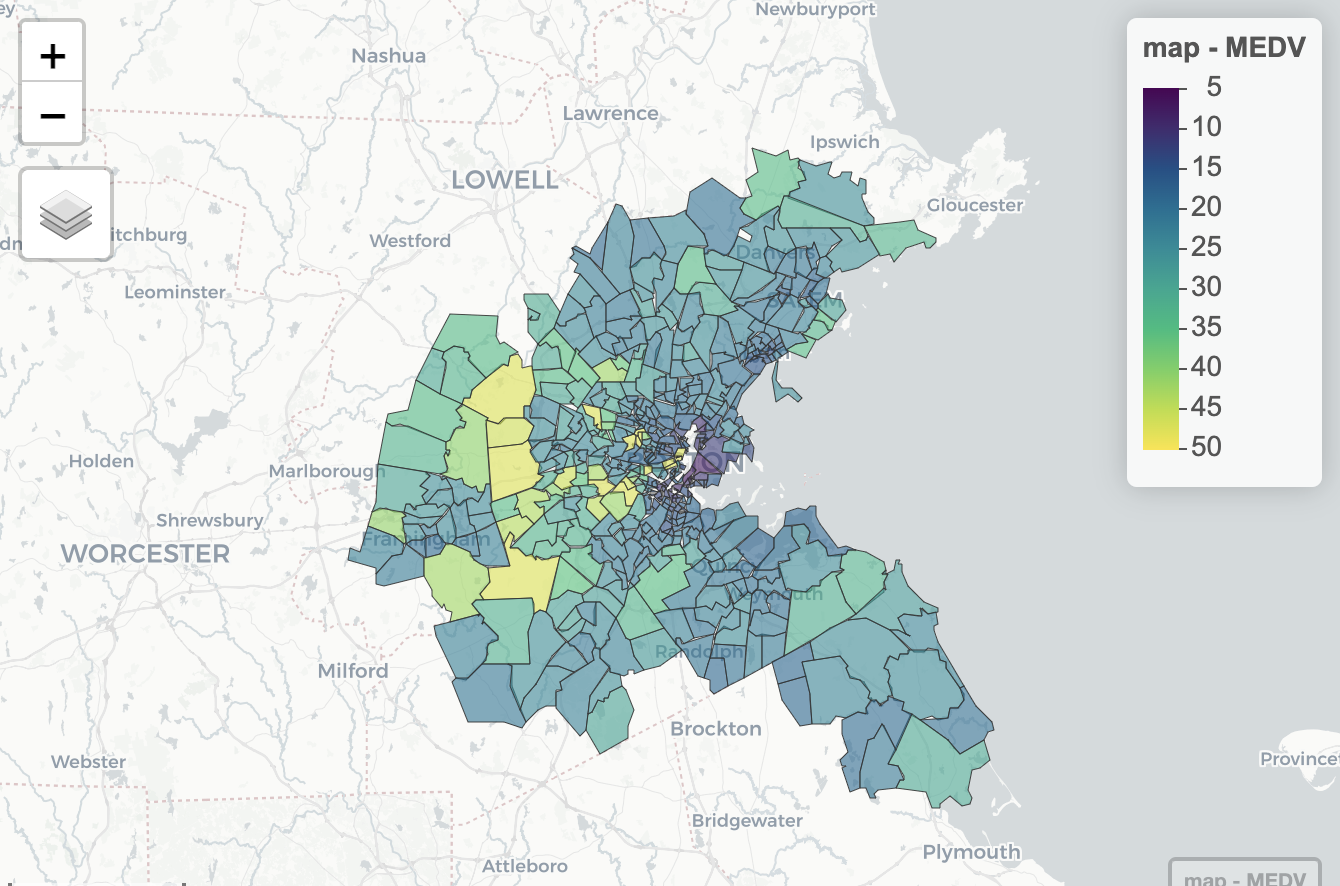
\includegraphics[height=75mm]{prices.png}
  \caption{Median Housing Price}
  \medskip
	\small
	The median house value (in \$1000USD) by census tract in the Greater Boston Area.
  \label{fig:prices}
\end{figure}

\begin{figure}[h!] 
  \centering
  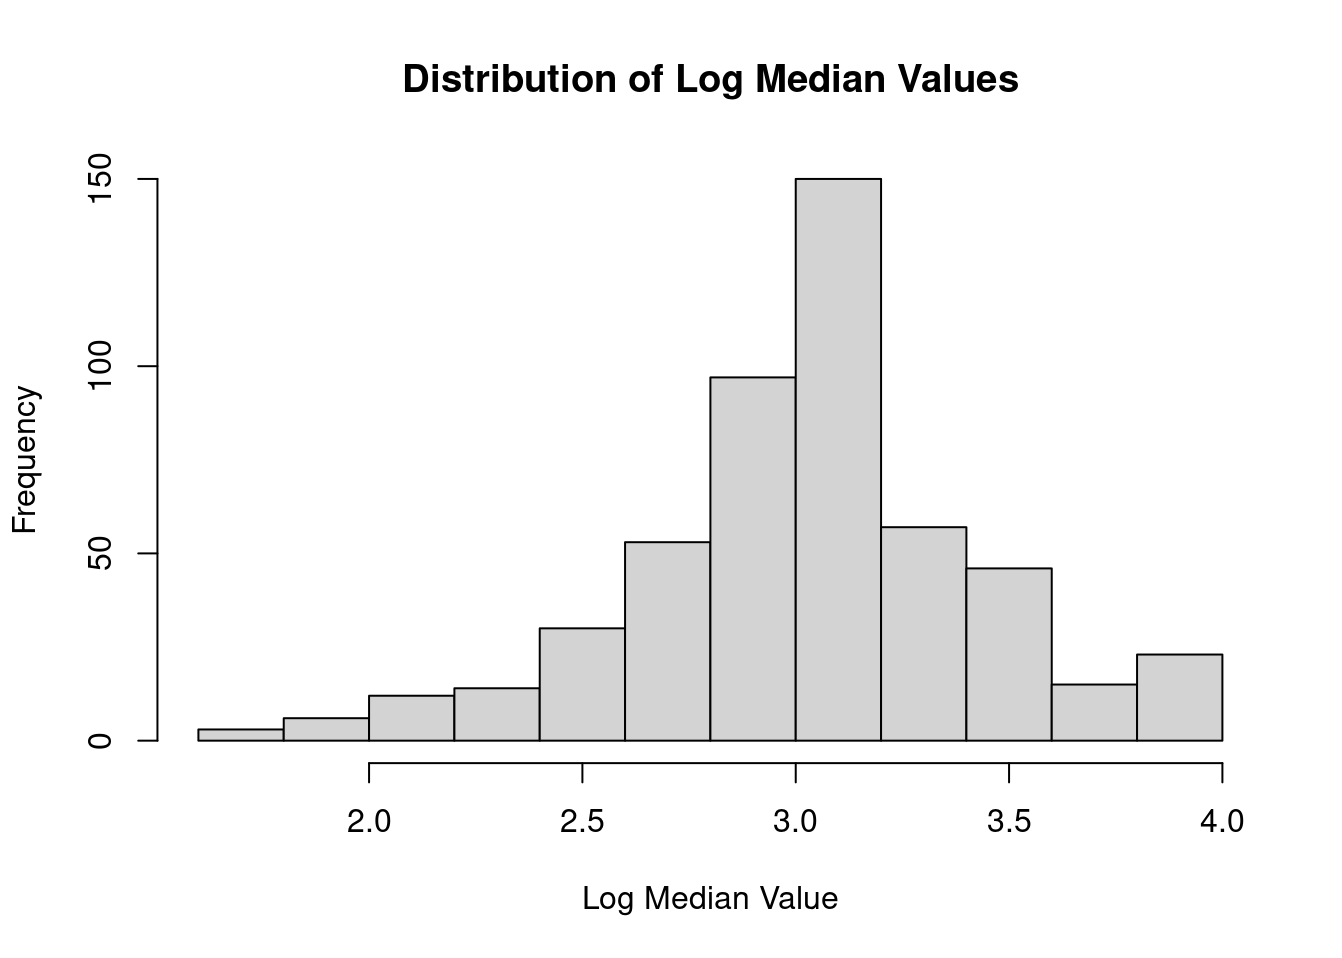
\includegraphics[height=75mm]{price_dist.png}
  \caption{Log Median Housing Price Distribution}
  \label{fig:price_dist}
\end{figure}


\begin{figure}[h!] 
  \centering
  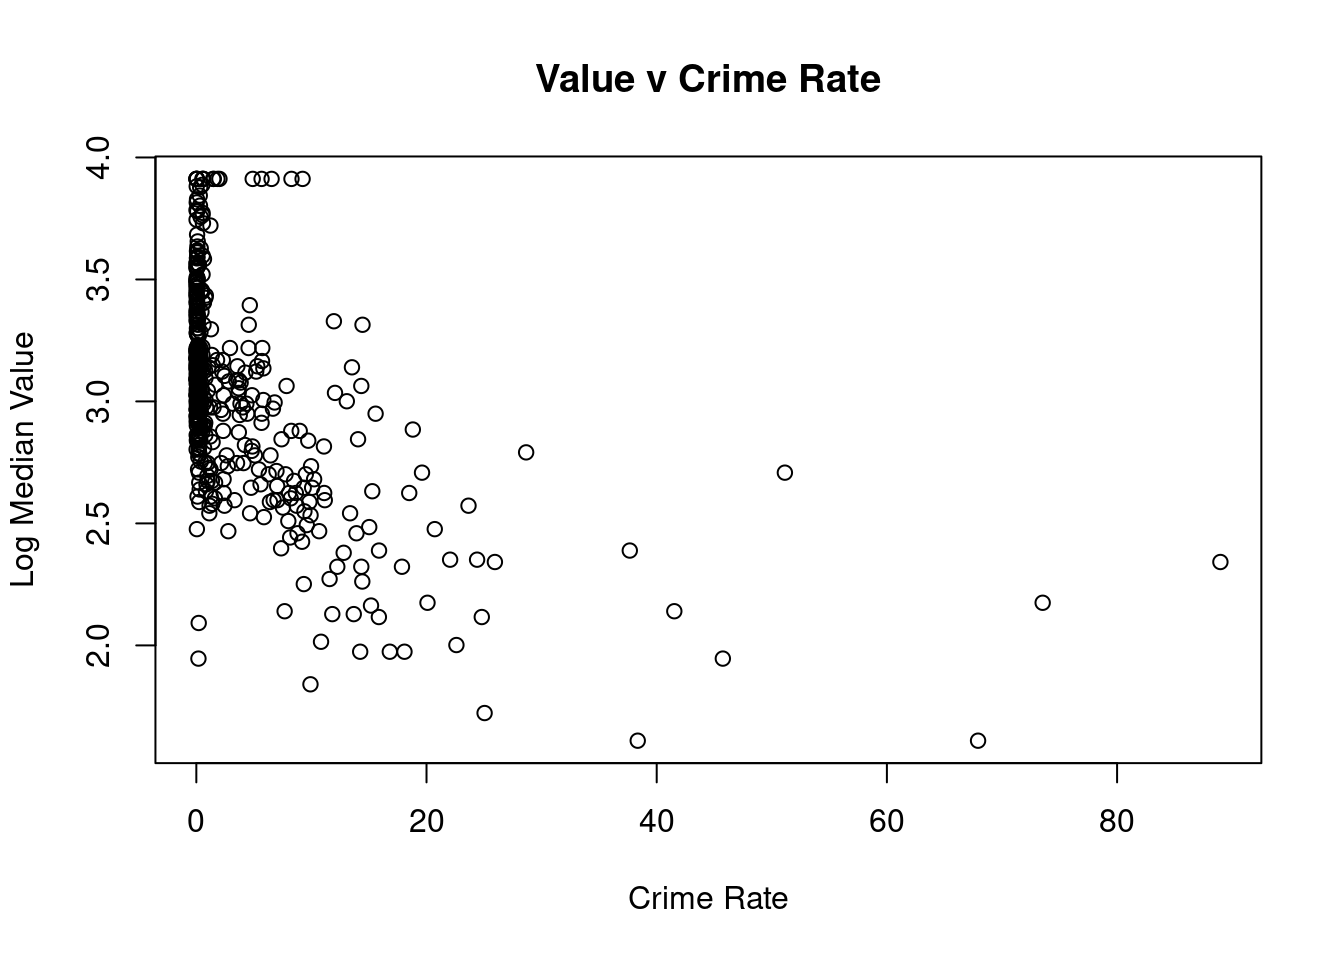
\includegraphics[height=75mm]{crime.png}
  \caption{Log Median Price vs Crime Rate}
  \label{fig:crime}
\end{figure}

\begin{figure}[h!] 
  \centering
  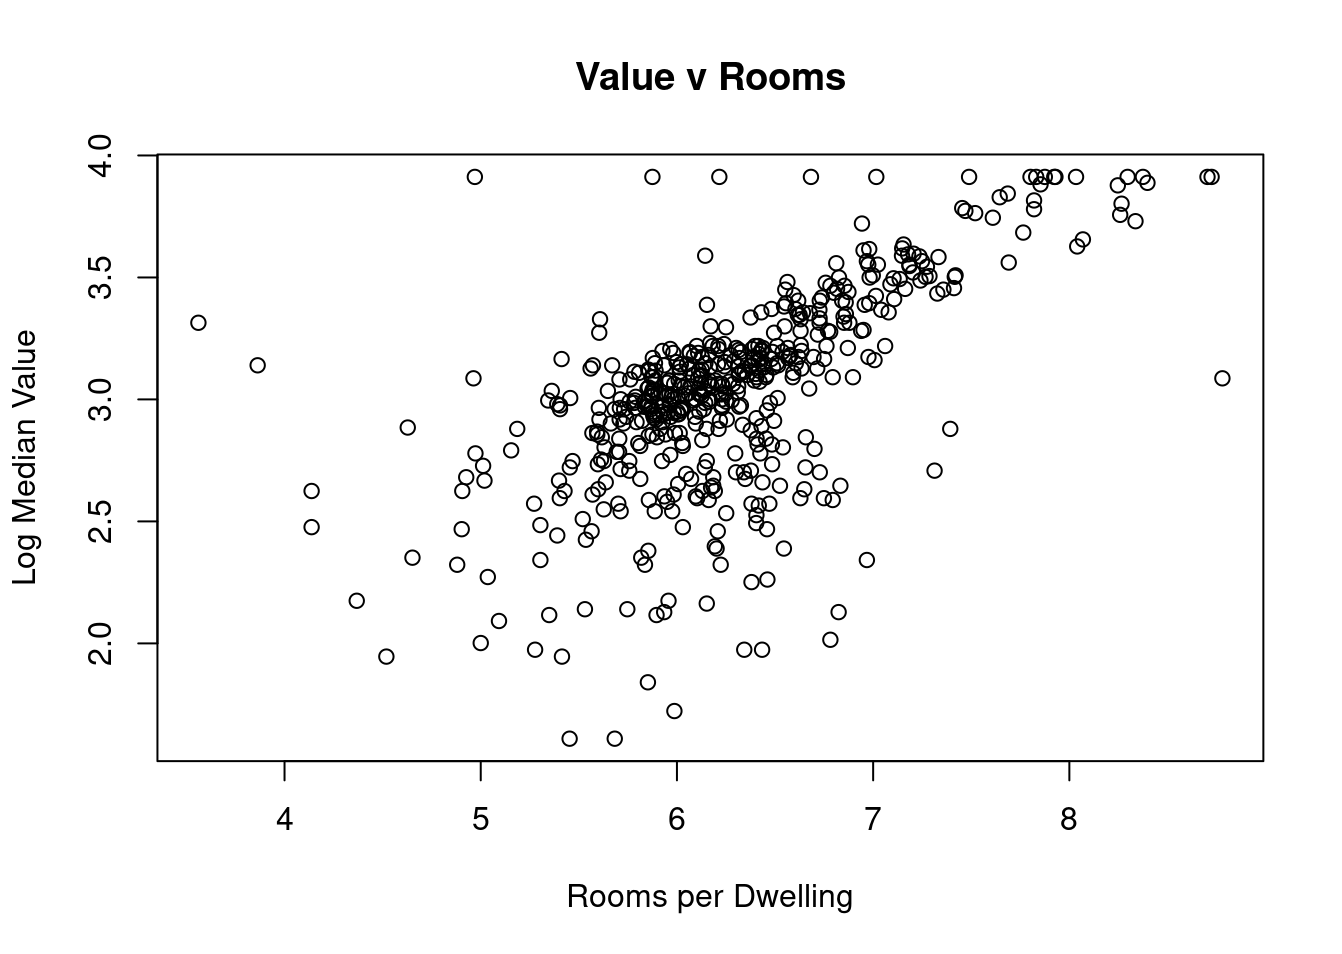
\includegraphics[height=75mm]{rooms.png}
  \caption{Log Median Price vs Rooms per Dwelling}
  \label{fig:rooms}
\end{figure}

\begin{figure}[h!] 
  \centering
  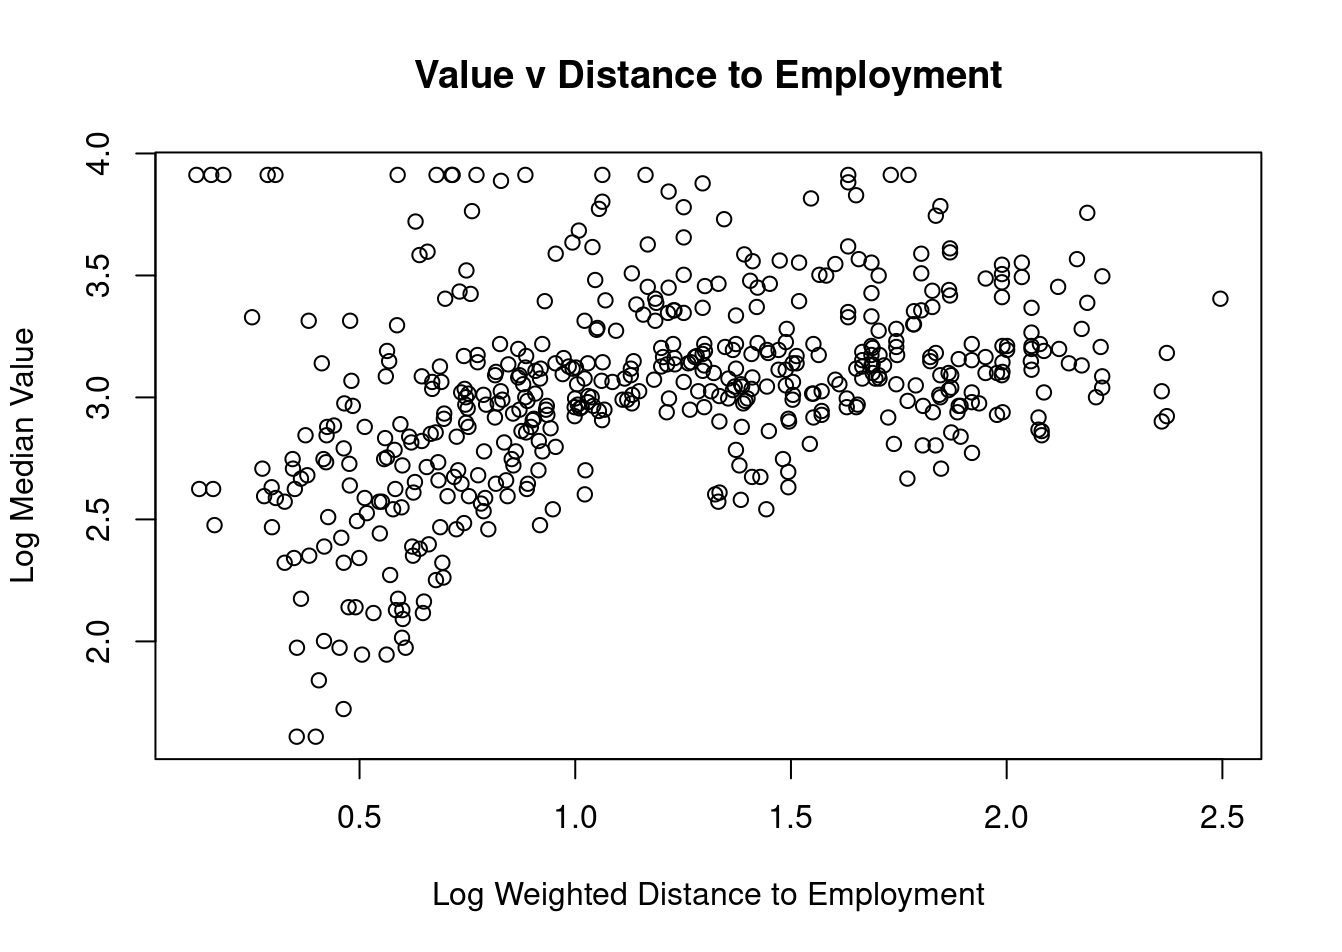
\includegraphics[height=75mm]{employment.png}
  \caption{Log Median Price vs Log Weighted Distance to Employment Centers}
  \label{fig:employment}
\end{figure}

\begin{figure}[h!] 
	\centering
  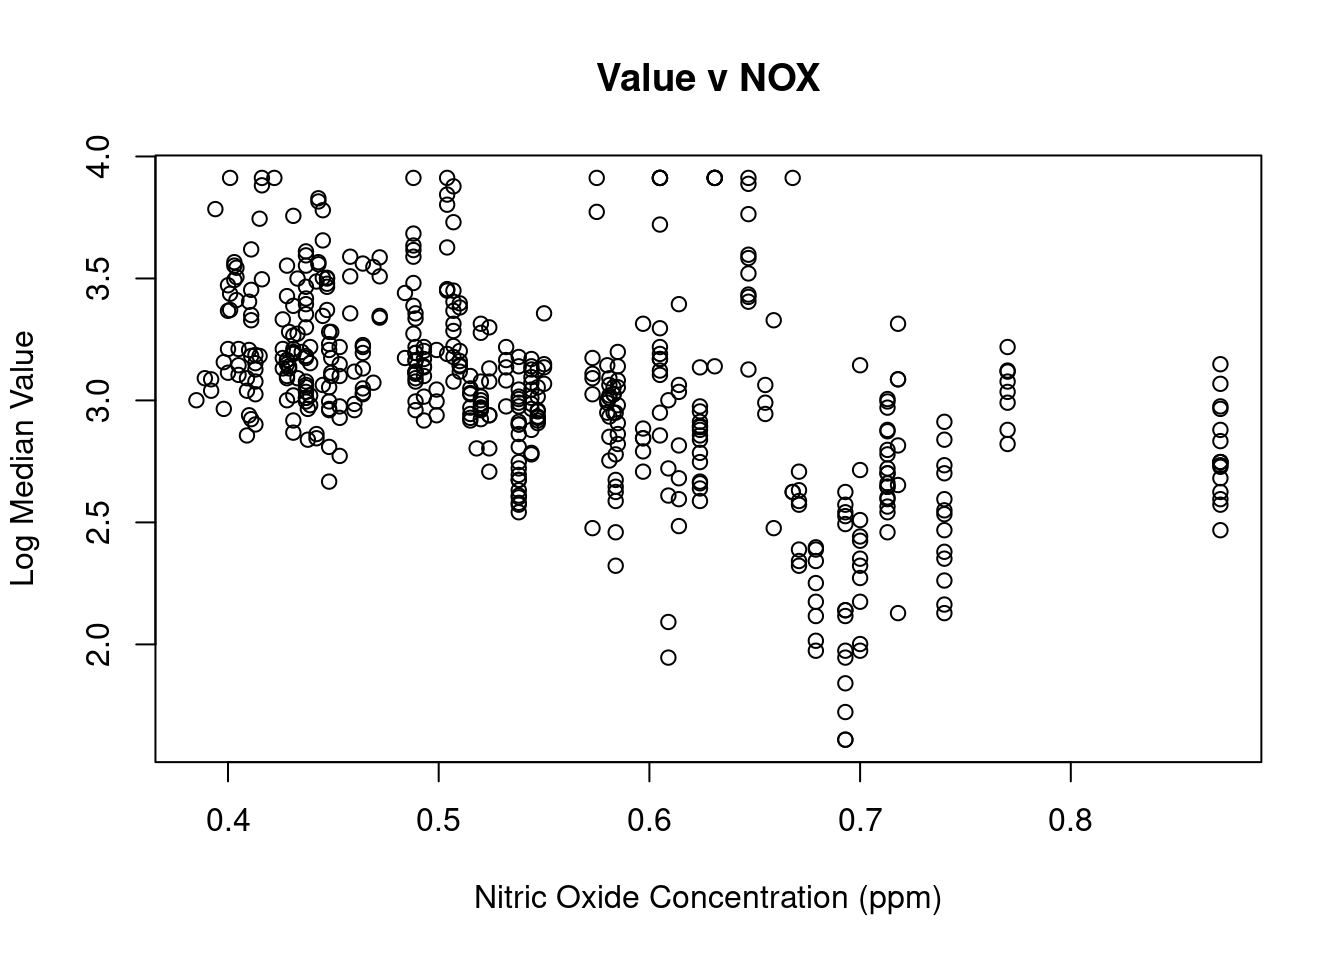
\includegraphics[height=75mm]{nox.png}
  \caption{Log Median Price vs NOX}
  \label{fig:nox}
\end{figure}


\begin{figure}[h!] 
	\centering
  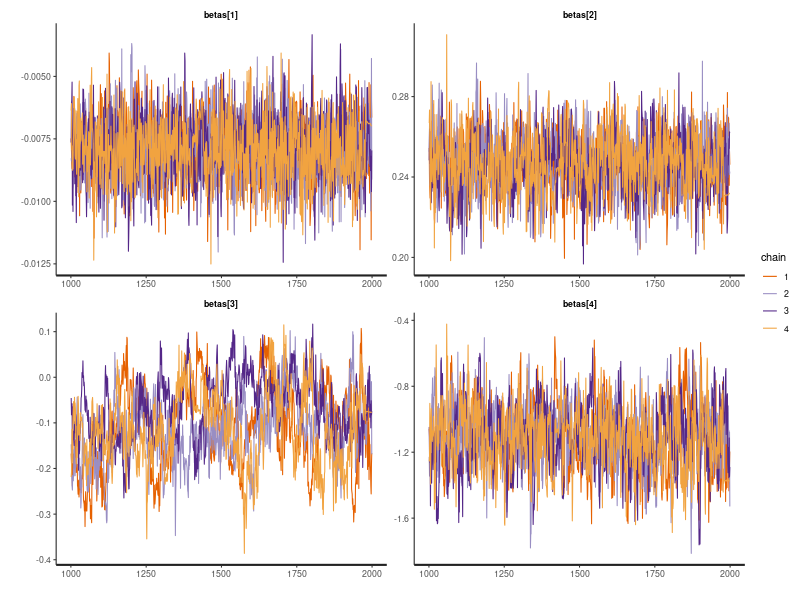
\includegraphics[height=75mm]{traceplot_betas.png}
  \caption{$\vec{\beta}$ Traceplots for 4 Feature Model}
  \label{fig:tbetas}
\end{figure}

\begin{figure}[h!] 
	\centering
  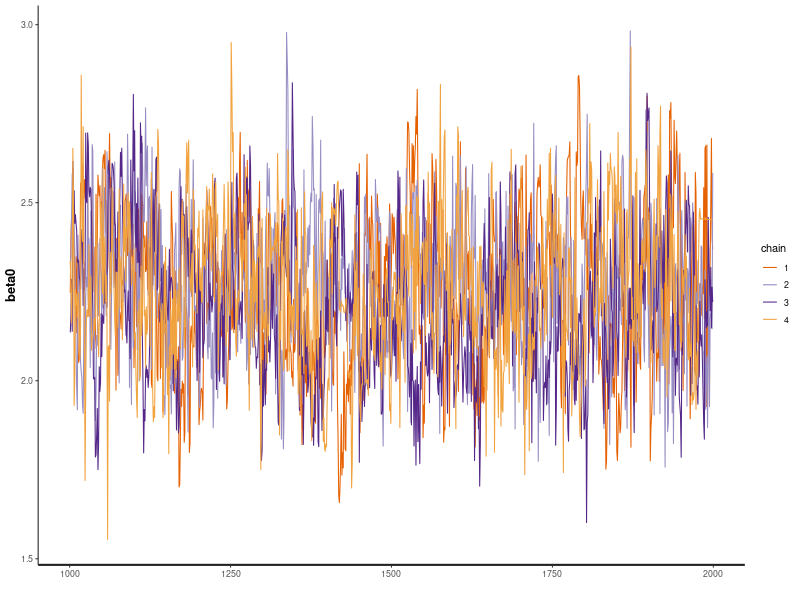
\includegraphics[height=75mm]{traceplot_beta0.png}
  \caption{$\beta_0$ Traceplot for 4 Feature Model}
  \label{fig:tbeta0}
\end{figure}

\begin{figure}[h!] 
	\centering
  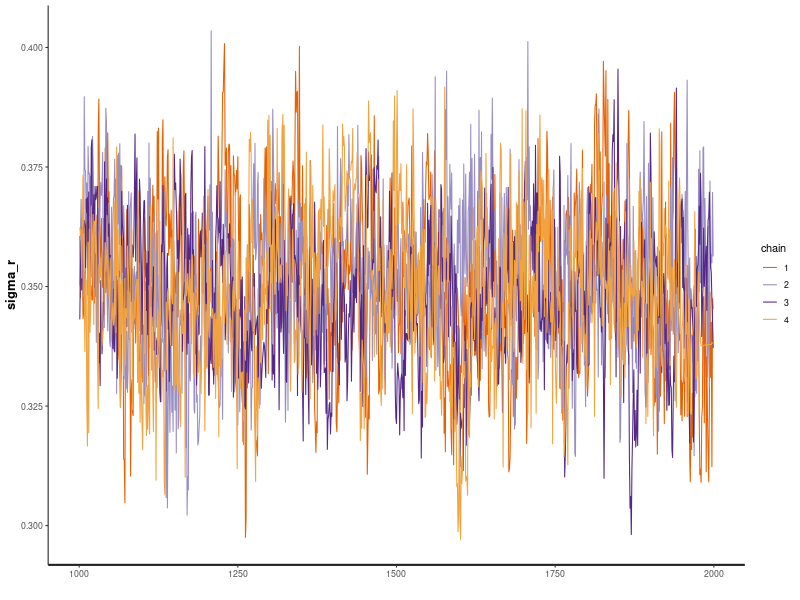
\includegraphics[height=75mm]{traceplot_sigma_r.png}
  \caption{$\sigma_r$ Traceplot for 4 Feature Model}
  \label{fig:tsigma_r}
\end{figure}

\begin{figure}[h!] 
	\centering
  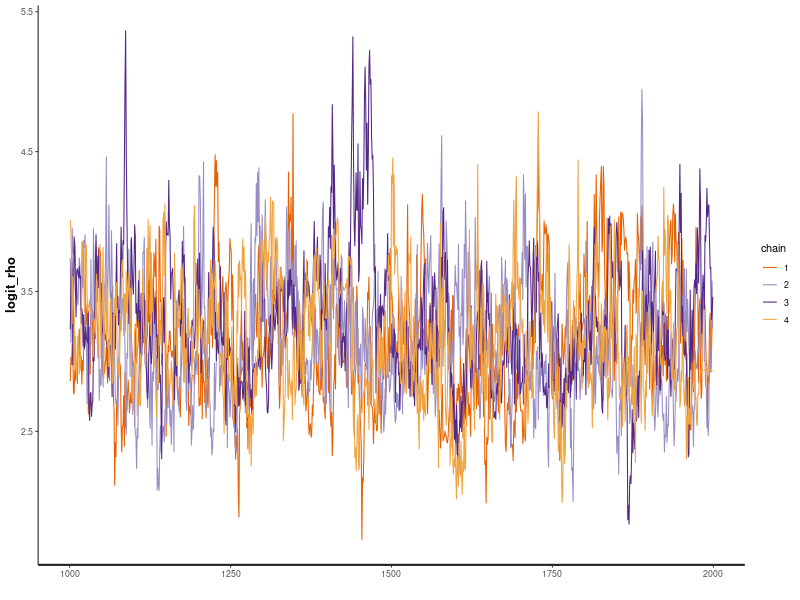
\includegraphics[height=75mm]{traceplot_logit_rho.png}
  \caption{$\rho$ Traceplot for 4 Feature Model}
  \label{fig:tlogit_rho}
\end{figure}



\begin{figure}[h!] 
	\centering
  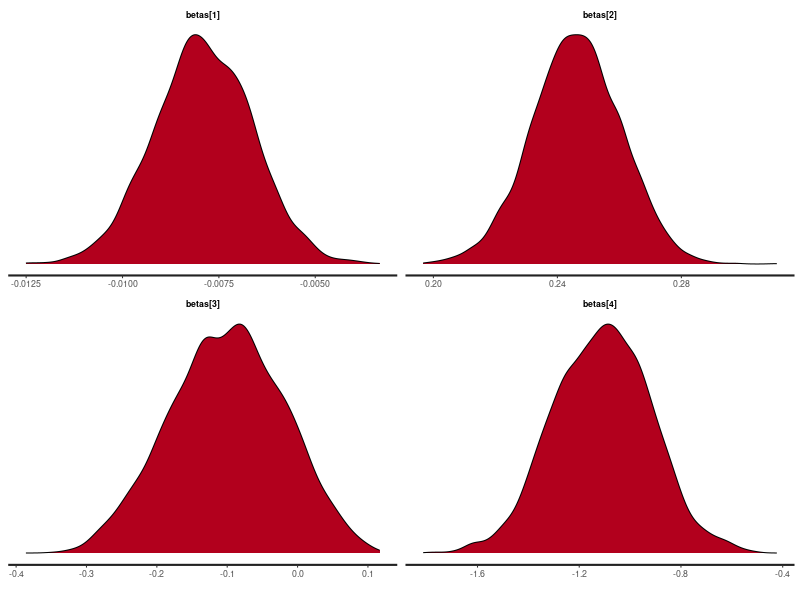
\includegraphics[height=75mm]{density_betas.png}
  \caption{$\vec{\beta}$ Densities for 4 Feature Model}
  \label{fig:dbetas}
\end{figure}

\begin{figure}[h!] 
	\centering
  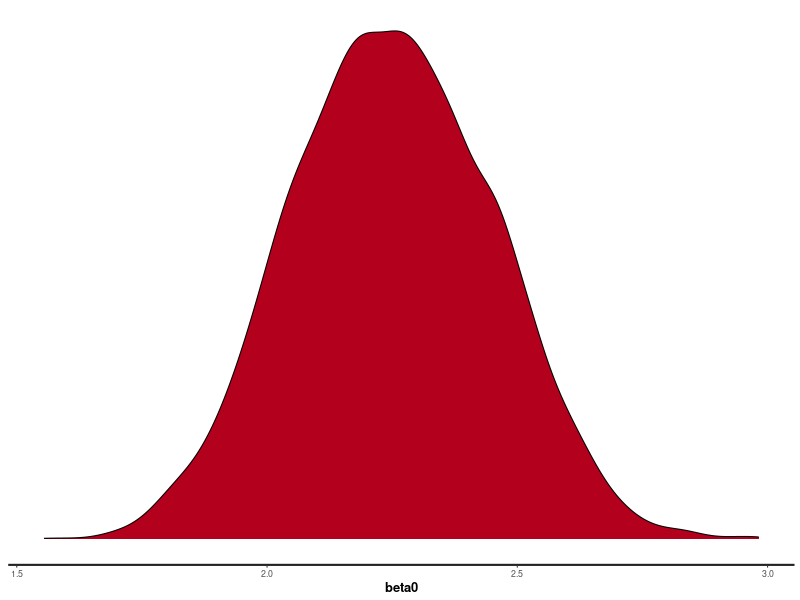
\includegraphics[height=75mm]{density_beta0.png}
  \caption{$\beta_0$ Density for 4 Feature Model}
  \label{fig:dbeta0}
\end{figure}

\begin{figure}[h!] 
	\centering
  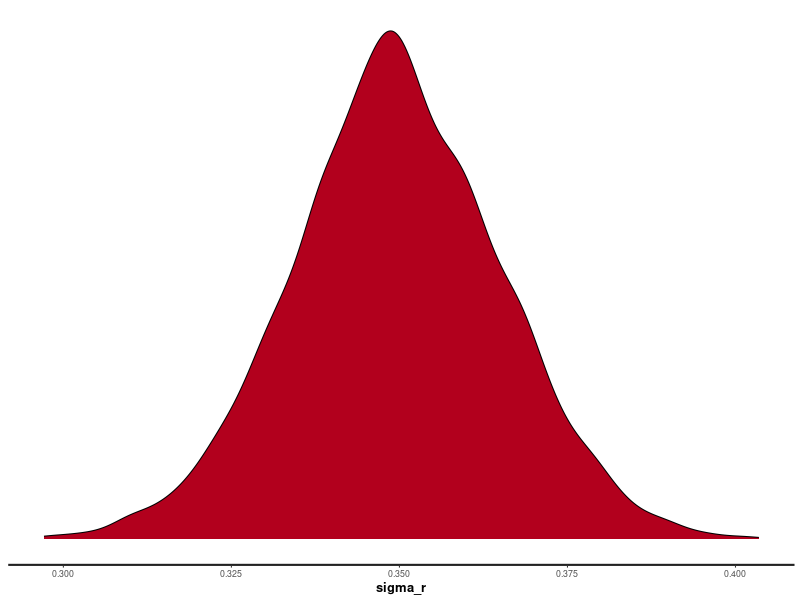
\includegraphics[height=75mm]{density_sigma_r.png}
  \caption{$\sigma_r$ Density for 4 Feature Model}
  \label{fig:dsigma_r}
\end{figure}

\begin{figure}[h!] 
	\centering
  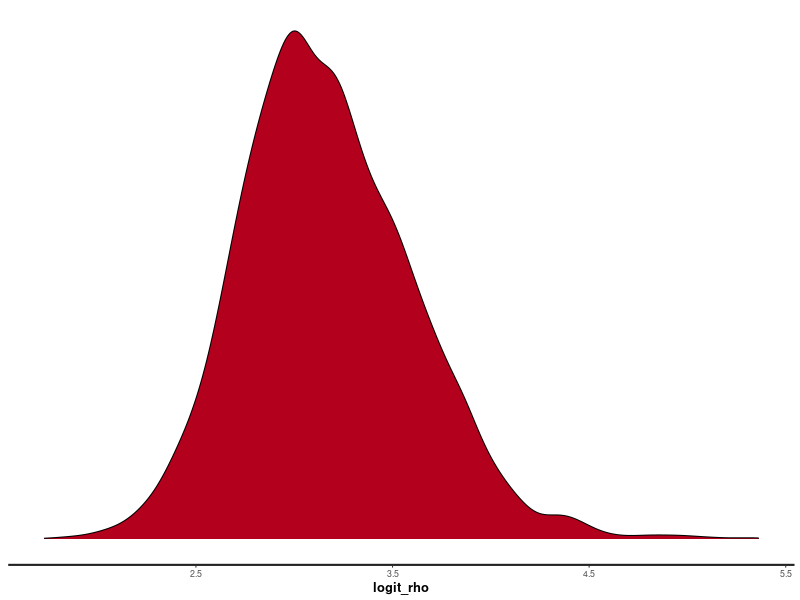
\includegraphics[height=75mm]{density_logit_rho.png}
  \caption{$\rho$ Density for 4 Feature Model}
  \label{fig:dlogit_rho}
\end{figure}












\begin{figure}[h!] 
	\centering
  \includegraphics[height=75mm]{traceplot_betas2.png}
  \caption{$\vec{\beta}$ Traceplots for 3 Feature Model}
  \label{fig:tbetas2}
\end{figure}

\begin{figure}[h!] 
	\centering
  \includegraphics[height=75mm]{traceplot_beta02.png}
  \caption{$\beta_0$ Traceplot for 3 Feature Model}
  \label{fig:tbeta02}
\end{figure}

\begin{figure}[h!] 
	\centering
  \includegraphics[height=75mm]{traceplot_sigma_r2.png}
  \caption{$\sigma_r$ Traceplot for 3 Feature Model}
  \label{fig:tsigma_r2}
\end{figure}

\begin{figure}[h!] 
	\centering
  \includegraphics[height=75mm]{traceplot_logit_rho2.png}
  \caption{$\rho$ Traceplot for 3 Feature Model}
  \label{fig:tlogit_rho2}
\end{figure}



\begin{figure}[h!] 
	\centering
  \includegraphics[height=75mm]{density_betas2.png}
  \caption{$\vec{\beta}$ Densities for 3 Feature Model}
  \label{fig:dbetas2}
\end{figure}

\begin{figure}[h!] 
	\centering
  \includegraphics[height=75mm]{density_beta02.png}
  \caption{$\beta_0$ Density for 3 Feature Model}
  \label{fig:dbeta02}
\end{figure}

\begin{figure}[h!] 
	\centering
  \includegraphics[height=75mm]{density_sigma_r2.png}
  \caption{$\sigma_r$ Density for 3 Feature Model}
  \label{fig:dsigma_r2}
\end{figure}

\begin{figure}[h!] 
	\centering
  \includegraphics[height=75mm]{density_logit_rho2.png}
  \caption{$\rho$ Density for 3 Feature Model}
  \label{fig:dlogit_rho2}
\end{figure}













\end{document}